\documentclass[a0paper]{tikzposter}

\usetheme{Steph}

% Packages
\usepackage[T1]{fontenc}
\usepackage[utf8]{inputenc}
\usepackage{natbib,mdframed,amsmath,calc,graphicx,amssymb,relsize,multirow,rotating,bm,url,multicol,array,subfigure,eurosym}
\usepackage{tikz}
\usetikzlibrary{arrows,patterns, calc, arrows.meta}
\tikzset{>={Latex[width=3mm,length=5mm]}}

\renewcommand{\rmdefault}{phv}
\renewcommand{\sfdefault}{phv} 
\renewcommand{\labelitemi}{$\bullet$}

\newcommand{\compresslist}{
    \setlength{\itemsep}{1pt}
	\setlength{\parskip}{0pt}
	\setlength{\parsep}{0pt}
}

\definecolor{IGNVert}{RGB}{163, 210,  11}
\definecolor{IGNGris}{RGB}{159, 164, 168}
\definecolor{IGNGrisFonce}{RGB}{101, 105, 110}

\graphicspath{./images}


\title{\textbf{Innovation dynamics in multi-scalar}}
\author{Juste Raimbault$^{1,\ast}$ and Denise Pumain$^2$}
\institute{$^1$ LASTIG, Univ. Gustave Eiffel, IGN-ENSG\\
$^2$ UMR CNRS 8504 Géographie-cités, Université Paris 1\bigskip\\
$\ast$ \texttt{juste.raimbault@ign.fr}}
\titlegraphic{}

% Layout of title and logos, some other possible logos are available in images folder
% Don't hesitate to modify the positions if it doesn't suit you
\makeatletter
\renewcommand\TP@maketitle{
    \hspace{-.12\textwidth}
	\begin{tabular}{lcl}
	%logo box 1
        
    	\begin{minipage}[b][.1\textheight][b]{.15\textwidth}
      
        	
\includegraphics[width=0.7\linewidth]{./figures/LOGO_IGN}\\
            
             \vspace{1cm}
            
            
\includegraphics[width=0.7\linewidth]{./figures/lastig}%\\
            
    	\end{minipage}
    	&
    	%title box
    	\begin{minipage}[b][.1\textheight][b]{.6\textwidth}

            
     
    		\centering
    		\color{titlefgcolor}
            \vspace{1cm}
    		{\bfseries \Huge \sc \@title \par}
    		
    		\vspace{-0.5cm}
    		{\bfseries \Huge \sc \textbf{systems of cities} \par}
    		\vspace*{2em}
    		{\huge \@author \par}
    		\vspace*{1em}
    		{\LARGE \@institute}
    		
    	\end{minipage}
    	&
    	%logo box 2
    	
    	\begin{minipage}[b][.1\textheight][b]{.15\textwidth}
    			
            	
\includegraphics[width=0.8\textwidth]{./figures/geocites.png}
    	\end{minipage}
	\end{tabular}
}
\makeatother

%%%%%%%%%%%%%%%%%%%%%%%%%%%%%%%%%%%%%%%%%%%%%%%%%%%%%%%%%%%%%%%%%%%%%%%%%%%%%%%%
% Multicol Settings
%%%%%%%%%%%%%%%%%%%%%%%%%%%%%%%%%%%%%%%%%%%%%%%%%%%%%%%%%%%%%%%%%%%%%%%%%%%%%%%%
\setlength{\columnsep}{1.5em}
\setlength{\columnseprule}{0mm}


% To remove the "latex tikz poster" at the bottom right corner
\tikzposterlatexaffectionproofoff

\begin{document}
	% Title block with title, author, logo, etc.
	\maketitle
	
%------------------------------------------------------
%----------------LINE 1--------------------------------
%------------------------------------------------------
	
	\begin{columns}
		
		\column{0.5}% Width set relative to text width

		
		%==============================================
		\block[titlewidthscale=0.7]{Urban dynamics and innovation}{

%Innovation is defined for social systems as inventions that became socially accepted, generating increasing returns and path dependence effects in territorial development \citep{arthur1994increasing}. Although inventions are not necessarily generated within cities, the processes of appearance and transmission of innovations are closely linked to urban development. Innovation and urban systems are thus two distinct dimensions of the Sustainable Development Goals which are tightly interlinked \citep{hegre2020synergies}. In a recent plea for better coordination of international development policies, \cite{keith2022new} emphasise that cities are drivers for the development of climate resilient approaches. Cities are complex adaptive systems whose size and functional specialization depend on their cumulative adaptation to the innovation they contribute to generate \citep{pumain2020theories}. Innovation remains rather highly geographically concentrated in an early stage before it becomes widely imitated and disseminated \citep{audretsch1996innovative}. Innovation clusters are indeed important components of local urban systems \citep{moreno2006innovation}. Spatial proximity favour local synergies, it supports knowledge spillover that may increase the spatial concentration and sustainability of innovation, provided that a related variety among local activities can help it \citep{boschma2009related,frenken2007related}.

%The scale of innovation processes became much more international in recent decades. Nowadays, the acceleration of global innovation is driven by two complementary processes: the action of major players such as multinational companies in their networks \citep{rozenblat2007firm}, and the connection of resources (such as knowledge, market access, financial investment and technology legitimacy) that had previously only been brought into contact to a limited extent. Systems of cities play a crucial role in innovation processes because of the multiple interactions they have developed over time \citep{scott2015nature}. Cities sizes inequalities are prone to enable complementarities that are helping the hierarchical diffusion of innovation \citep{hagerstrand1968innovation}. As confirmed by recent investigations in urban scaling laws \citep{pumain2006evolutionary}, innovative activities at first concentrate in higher levels of urban hierarchies where skills and diversity are maximised, in a second stage they relocate in medium size cities where labour and housing market are less expensive and in a third stage relatively concentrate in smaller places. Thus in general innovation diffusion dynamics imply multiple scales. Besides the multiple observations of local innovative milieu, and the quest for global innovation systems \citep{binz2017global}, there is a regionalisation process that encourage developmental transnational partnerships between countries that belong to different regions of the world experimenting similar problems, as in the EU \citep{palle2022multilevel} or ASEAN in South Asia \citep{krapohl2017regional}. \cite{binz2017global} suggest a typology of global innovation systems based on the type of linkages within and between scales, from the regional to the global one, with different policy implications to encourage green technologies. \cite{bauer2019local} show that the interplay between local innovation and global trends is crucial for the clean transition of chemical industries.



          \vspace{0.35cm}
            
			\begin{itemize}
				\item Cities are central for innovation in social systems \cite{pumain2020theories} and future sustainability \cite{keith2022newshort}
                 \vspace{0.35cm}
				\item Urban innovation systems now span from local clusters to global networks
				\vspace{0.35cm}
				\item Innovation dynamics in systems of cities follow complex patterns across scales
				\vspace{0.35cm}
			\end{itemize}
		}
		%==============================================
		
		% Second column on same line than first one
		\column{0.5}
	    %==============================================
		\block[titlewidthscale=0.7]{Towards multi-scalar models}{


%Multi-scalar approaches are therefore necessary for innovation policies and governance. Modelling and simulation are in that context a privileged tool to understand system dynamics and elaborate policies. \cite{rozenblat2018conclusion} emphasise the need for multi-scalar models for sustainable territorial policies. The field of artificial life (ALife) has an important contribution record to the simulation of social systems, including for example the stock market \citep{palmer1994artificial}, social interactions \citep{sawyer2003artificial}, sustainable cities \citep{wang2004artificial}. One advantage of such ``artificial societies'' approaches is that they provide some explanatory power through their generative aspect \citep{grune2009explanatory}. The quantitative study of cities and urban systems has always kept tight links with ALife \citep{raimbault2020cities}. Recent urban simulation examples include the simulation of urban morphology \citep{raimbault2019generating} or informal innovation diffusion in firm clusters \citep{raimbault2022innovation}. Multi-scale models have also been proposed in that context, such as by \cite{raimbault2021strong} which couple population dynamics in a system of cities with local urban form dynamics. \cite{raimbault2021multiscale} simulates building evolution at one scale and transportation network dynamics at one other. \cite{rojas2021sustainability} introduces a network model for the diffusion of renewable energy technologies with applications at multiple scales. \cite{torrens2012polyspatial} use agents which can act at different scales to capture multi-scalar aspects of urban growth. Urban climate is also an aspect requiring highly resolved local models which can be integrated into broader meteorological models \citep{mauree2018multi}. Other aspects of social interactions, such as epidemiological modelling, are also cases where coupling between scales allows refining macroscopic equation models \citep{banos2015importance}. In the case of urban dynamics modelling, the diversity of processes and actors acting at distinct scales makes it complicated to build multi-scalar models (need for distinct ontologies and specific processes to capture the feedback between scales \citep{raimbault2021strong}), on the contrary to other types of system where the links are more explicit such as traffic \citep{banos2017multiscale}.

%This paper proposes to investigate a social simulation approach to multi-scalar innovation dynamics in systems of cities. We study how the macroscopic scale of regional systems can be articulated with the mesoscopic scale of urban areas, for the emergence of new innovations within research clusters and the diffusion of these innovations between cities. We focus on the feedback between scales, the autonomy of each scale, and the need to build such a ``complicated'' model to capture strong emergence. Our contribution relies more precisely on the following: (i) we build a multi-scalar agent-based model for innovation dynamics, by coupling an innovation cluster model with an urban dynamics model at the macroscopic scale - based on existing models which have been modified and extended with some coupling processes between scales - and that we apply on synthetic systems of cities with a realistic geographical setting; (ii) we explore the coupled model parameter space using the OpenMOLE platform for model validation, including a bi-objective optimisation between utility at the macro scale and diversity at the meso scale; (iii) we implement indicators to quantify downward causation in order to understand the complexity of inter-scale interactions; (iv) we apply a diversity search algorithm to find how flexible the model is to generate ``regimes of emergence''.

%The rest of the paper is organised as follows: we first formally describe the simulation model and its parametrisation; we partly validate the model by sampling its parameter space to study its statistical properties and indicator behaviour; we then run a bi-objective optimisation to find compromise between objectives at different scales; we describe the regimes of emergence obtained with the diversity search algorithm; we finally discuss the implications of our results and perspectives open for future work.

           
           % \vspace{0.3cm}
            
			\begin{itemize}
				\item Multi-scalar models necessary to design sustainable territorial policies \cite{rozenblat2018conclusion}
                %\vspace{0.3cm}
				\item ``Artificial cities'' \cite{raimbault2020cities} and urban simulation approaches focus on a single scale
			\end{itemize}
			
			$\rightarrow$ a new \textbf{simulation model} coupling innovation diffusion dynamics \textbf{between cities} (macro) \cite{raimbault2020modelshort} with research cluster dynamics \textbf{within urban areas} (meso) \cite{raimbault2022innovationshort}
		
		}
		%==============================================
		
		%==============================================
		%end of first line
	\end{columns}
	
%------------------------------------------------------
%----------------LINE 2--------------------------------
%------------------------------------------------------

% block alone on its line so you don't have to specify the columns environment

		%==============================================
		\block[titlewidthscale=0.25]{Simulation model}{


% Our main hypothesis to build this model is that two distinct scales and dynamics, strongly coupled through bottom-up and top-down feedback, are necessary to capture the whole complexity of innovation systems. At the macroscopic scale of systems of cities, important related processes are the hierarchical diffusion of innovations between urban areas \citep{hagerstrand1968innovation} and the economic specialisation of these areas. \cite{favaro2011gibrat} proposed an urban dynamics model focusing on innovation diffusion, which was extended into an urban evolution model by \cite{raimbault2020model}. At the mesoscopic scale of innovation clusters, firms interact directly but also informally, and the innovation dynamics within a local area will be driven, beside numerous economic factors, by the exchange of ideas and research dynamics within and between firms (including academic bodies). \cite{raimbault2022innovation} introduced a simple model of firm clusters, accounting for geographical structure and the flow of ideas between firms, similar to a biogeography optimisation algorithm \citep{simon2008biogeography}. The multi-scale model we propose is based on a strong coupling between the macroscopic agent-based model of \cite{raimbault2020model} and the mesoscopic agent-based model of \cite{raimbault2022innovation}. Innovations diffuse within an urban system with several urban areas, in which firms search for new innovations. To simplify, urban areas are isolated enough so that no innovation cluster extends on two distinct areas (what is geographically reasonable for most worldwide urban systems, besides polycentric mega-city regions- which should in our case be considered as a single urban area \citep{yeh2020cities}). We assume a certain independence between the macro and meso dynamics, as they have each their own processes: innovation diffusion, adoption by the population, urban migration and growth, for the macro-scale; and flows of ideas within and between firms, mutation of ideas, multi-dimensional problem solving, for the meso scale. The link between scales is ensured through a bottom-up feedback: fitness performances of a local cluster, within a local innovation cycle corresponding to a macro time step, will determine the emergence of new innovations (replacing the mutation mechanism of the urban evolution model of \cite{raimbault2020model} we integrate); and through a top-down feedback: after a macro time-step, city population growth - interpreted as a global performance proxy - will have an impact on the strategies of firms and on the local urban environment, what is captured by a modification of parameter values of mesoscopic models.

% At the macroscopic scale, agents in the model are $N$ urban areas indexed by $i$, characterised by their population $P_i(t)$ evolving with time $t\geq t_0$ and innovation genome $\delta_{ic}(t)$ which corresponds to the share of different innovations (indexed by $c$) adopted in each area. For the geographical configuration, we work on synthetic systems of cities with realistic properties, what allows exploring model behaviour independently of geographical contingencies \citep{raimbault2019space}. Initial cities sizes in terms of population follow a rank-size law (Zipf's law) $P_i = P_0 \cdot i^{-\alpha^P}$, with $P_0$ the size of the largest city, $i$ the rank in decreasing order, and $\alpha_P$ the hierarchy \citep{ioannides2003zipf}.

%The mesoscopic geographical scale corresponds to the internal representation of each area, which consists in a cluster of firms. The number of firms $N_i$ in each area scales with city size \citep{pumain2006evolutionary}, such that $N_i = N_0 \cdot \left(\frac{P_i (t_0)}{P_0 (t_0)}\right)^{\alpha_N}$. We furthermore consider a global rank-size law for the size of firms (number of employees), in accordance with the empirical literature \citep{axtell2001zipf}, given by $S_k = S_0 \cdot k^{- \alpha_S}$, where $k$ is sorted in decreasing order, and such that $1 \leq k \leq \sum_i N_i$. To distribute initial firms into the urban areas: (i) we assume that the size of the largest firm scales with city size $\max_{k\in i} S_k = S_0 \cdot k^{- \alpha_L}$; (ii) sampling the set of all firms previously generated, we select for each area its largest by choosing the one with a size closest to the one given by the previous law; (iii) remaining missing firms are uniformly drawn within the sample of firms smallest than the largest, starting with the smallest urban area such that all firms are distributed in the end.

%Each innovation cluster is initialised with random employees within each firm (an employee corresponding to a set of ideas, i.e. a multidimensional genome), and with a random fitness to maximise following \cite{raimbault2022innovation} given by a generalised Rastrigin function $y(\vec{x}) = - \sum_{i,j} m_{ij} \left[x_i^2 - 10 \cos\left(2 \pi x_i\right) \right] $ for an employee ideas $\vec{x}$ and $m_{ij}$ uniformly drawn random coefficients. Such difficult optimisation landscapes have been used in the literature as a proxy of what firms seek to optimise. Firms have uniformly distributed locations within each area. Each area has its own meso parameters (listed below), initialised at the same value but evolving in different ways with the macro trajectory of the city.



            \begin{multicols}{3}
            
            Synthetic \textbf{system of cities} with populations following a Zipf law and random positions in the geographical space; within each city an \textbf{innovation cluster} is composed of firms, themselves composed by employees (ideas as real-valued genome), which aim at optimising a fixed random fitness (Rastrigin function).
            
            \vspace{1.5cm}
            
            \textbf{Iterated steps}, for $t_f$ macro time steps:
            \begin{enumerate}
\item \textbf{Meso cycle:} in each cluster for $t_m$ meso time steps:
    \begin{itemize}
        \item employee exchange ideas within firms (genome crossovers)
        \item idea with best fitness is chosen by each company
        \item ideas are informally exchanged between firms
    \end{itemize}
\item \textbf{Bottom-up feedback:} if relative fitness gain of the best firm exceeds a parameter  ($\delta f_i > \theta$), the corresponding city will innovate at the macro scale.
\item \textbf{Macro step:} innovation are diffused between cities; population migration and growth follow spatial interactions based on attractivity; new innovations are added to cities' genomes.
        
\item \textbf{Top-down feedback:} firm strategy is updated by changing crossover probability and mutation probability, and the urban environment in terms of informal exchanges, both depending on relative population growth.
\end{enumerate}
            
            \vspace{1.5cm}
            
            \textbf{Indicators:}
            \begin{itemize}
            	\item Macro observables: utility and diversity of innovations
            	\item Meso observables: best fitness and diversity of ideas
            	\item Indicators for downward causation from \cite{rosas2020reconcilingshort} ($\Delta$, $\Psi$, $\Gamma$) on these observables to quantify the strength of emergence
            \end{itemize}
            
             \vspace{1.5cm}
             
             \textbf{Implementation:}
             \begin{itemize}
             	\item Model implemented in scala: \url{https://github.com/JusteRaimbault/InnovationMultiscale-model}
             	\item Integrated into the OpenMOLE platform for model exploration and validation	\cite{reuillon2013openmole}
             \end{itemize}

            	
            \end{multicols}

   
		}
		
		
	
%------------------------------------------------------
%----------------LINE 3--------------------------------
%------------------------------------------------------

	
	\begin{columns}
		
		\column{0.5}% Width set relative to text width

		
		%==============================================
		\block[titlewidthscale=0.4]{Model exploration}{

            \parbox{0.6\linewidth}{
              
              \vspace{1cm}
              
              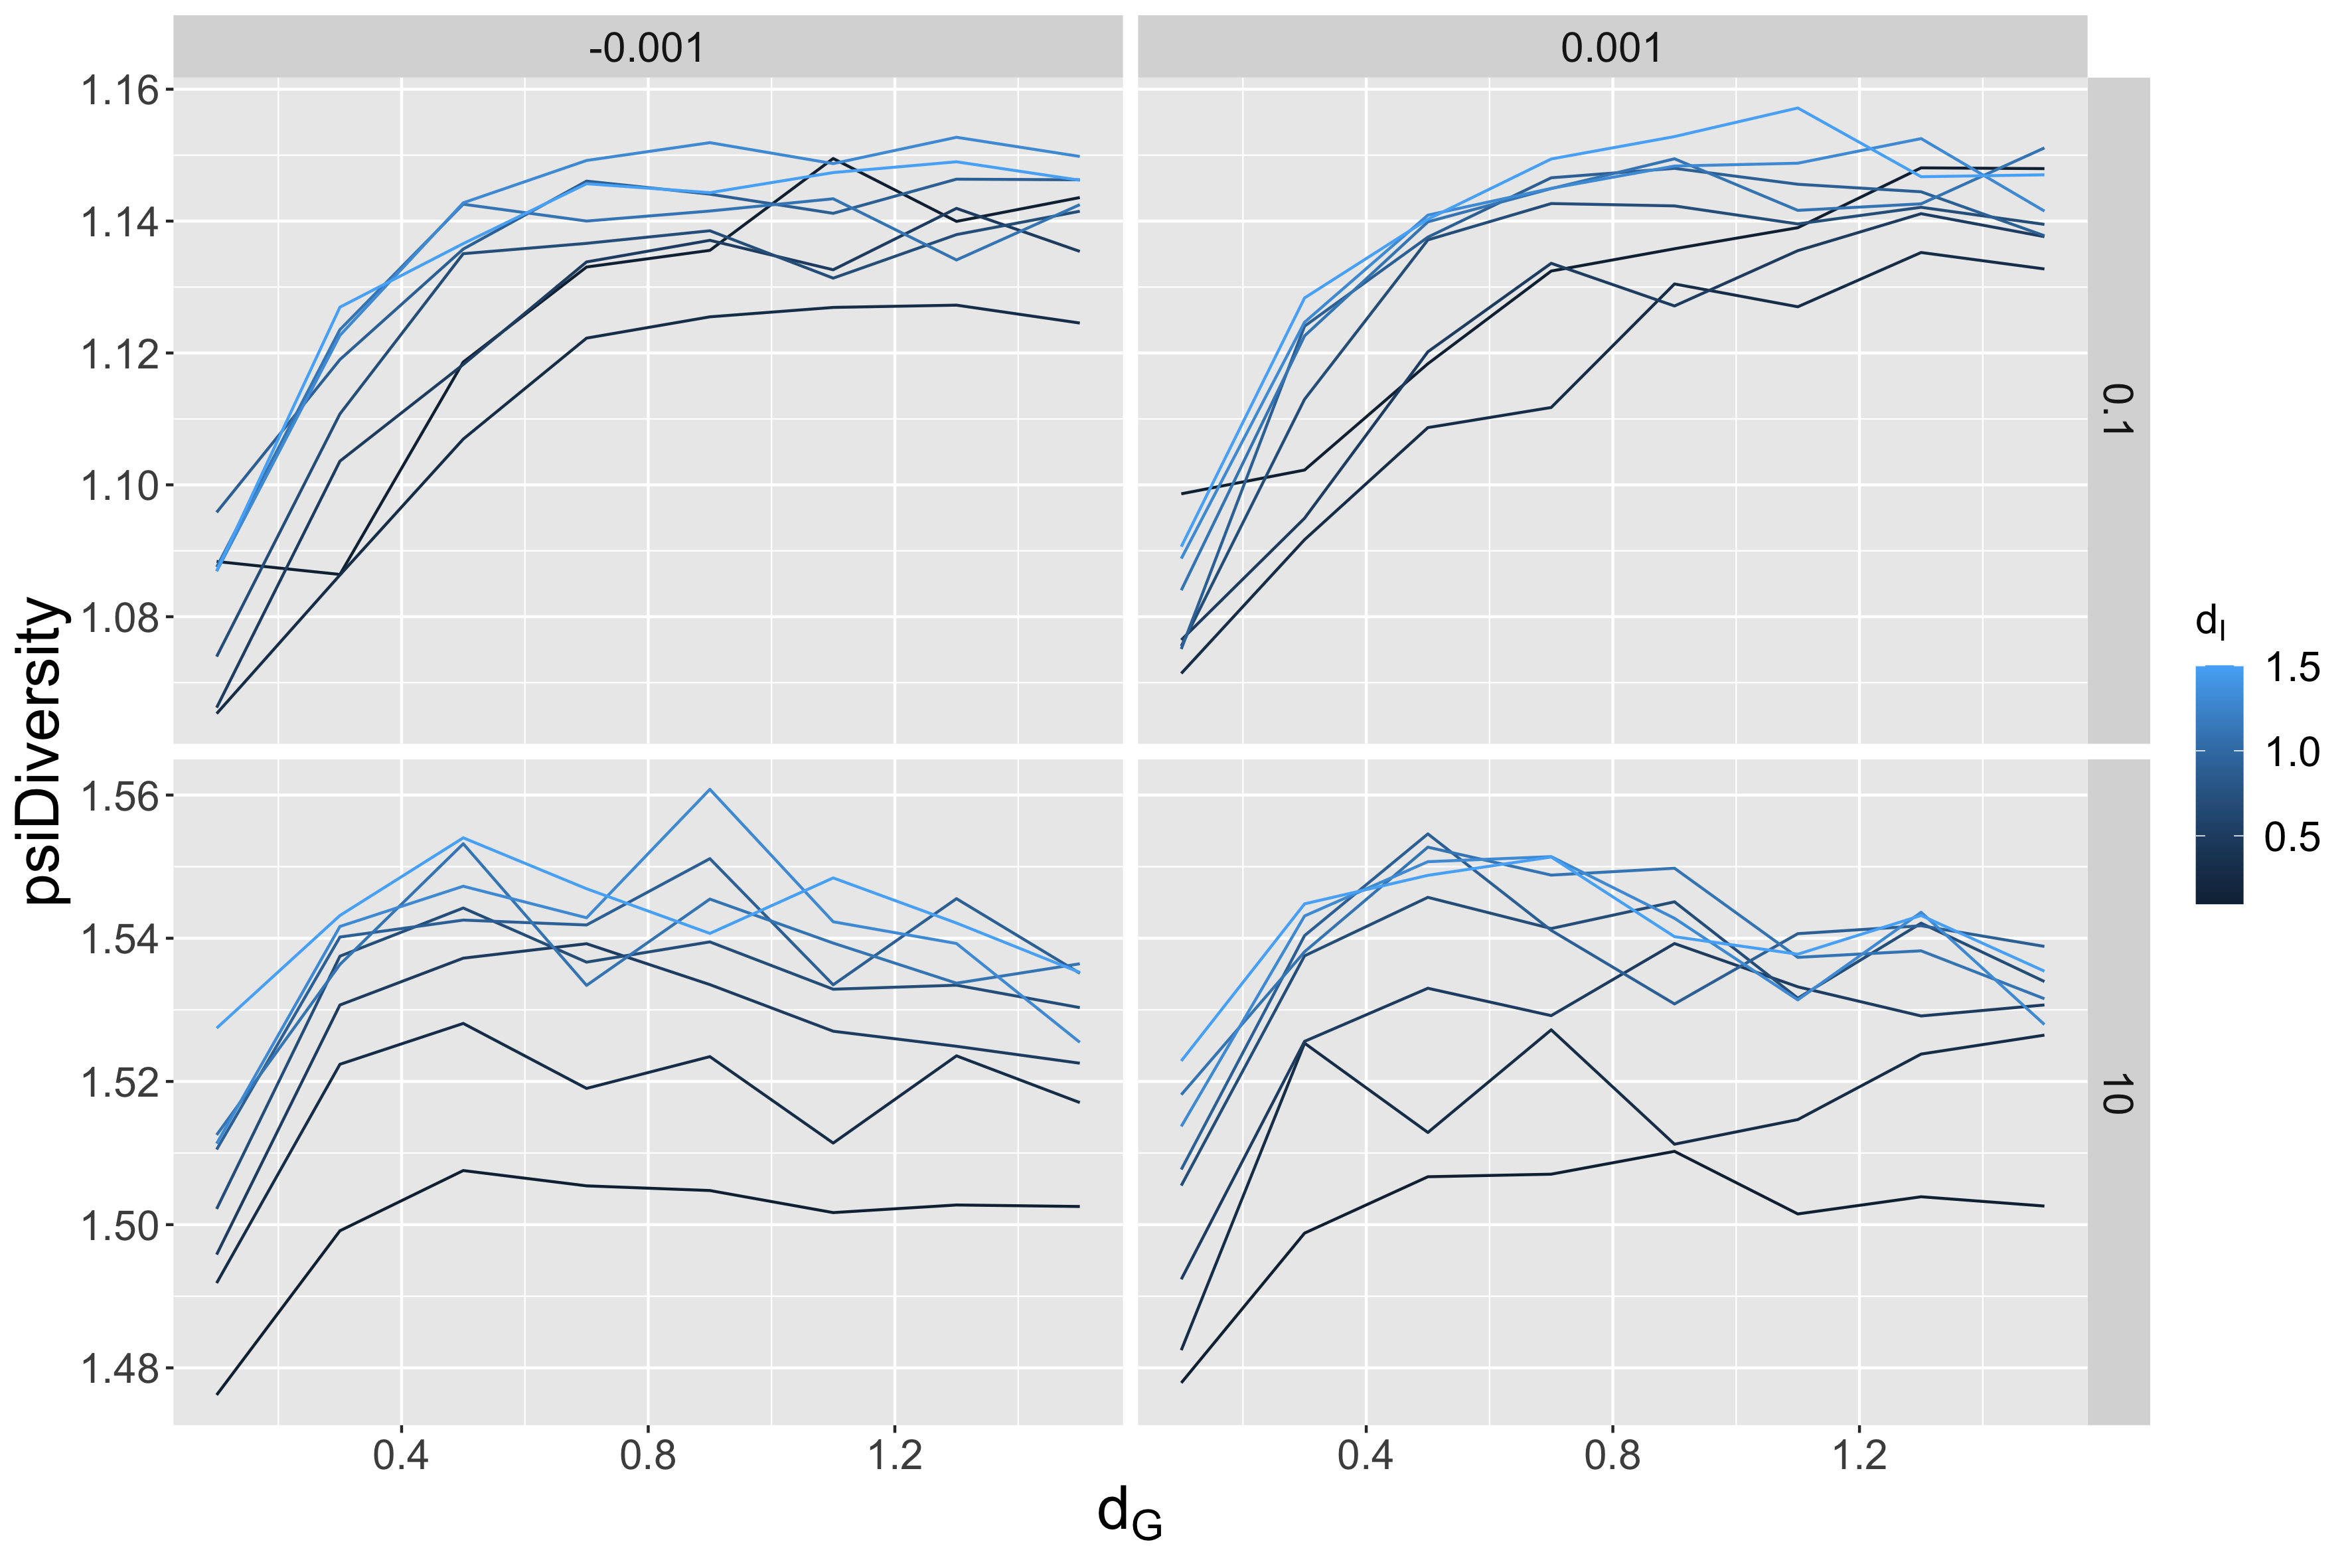
\includegraphics[width=\linewidth]{figures/psiDiversity-macroGravityDecay_color-macroInnovationDecay_facet-mesoToMacroInnovationThreshold-macroToMesoExchangeMaxUpdate_mesoCrossOverProba0-5.png}
              
		      }
            \hspace{0.5cm}
            \parbox{0.37\linewidth}{
			    
			   \textbf{Grid exploration} of the parameter space, to explore main dynamics of the model; 10,000 replications for each parameter point; variety of indicator behaviours.
			   
			    \vspace{0.5cm}
			  
			    
			    \textit{Left plot:} increasing then plateauing strength of emergence $\Psi$ for macro diversity, as a function of spatial interaction range $d_G$ and innovation diffusion range $d_I$, for varying top-down (columns) and bottom-up (rows) feedbacks.
			    
			     %\vspace{0.5cm}
			    
			     %$\rightarrow$ variety of 
			     
		      }
			
			
			
		}
		%==============================================
		
		% Second column on same line than first one
		\column{0.5}
	    %==============================================
		\block[titlewidthscale=0.4]{Optimisation}{

           \parbox{0.5\linewidth}{
              
              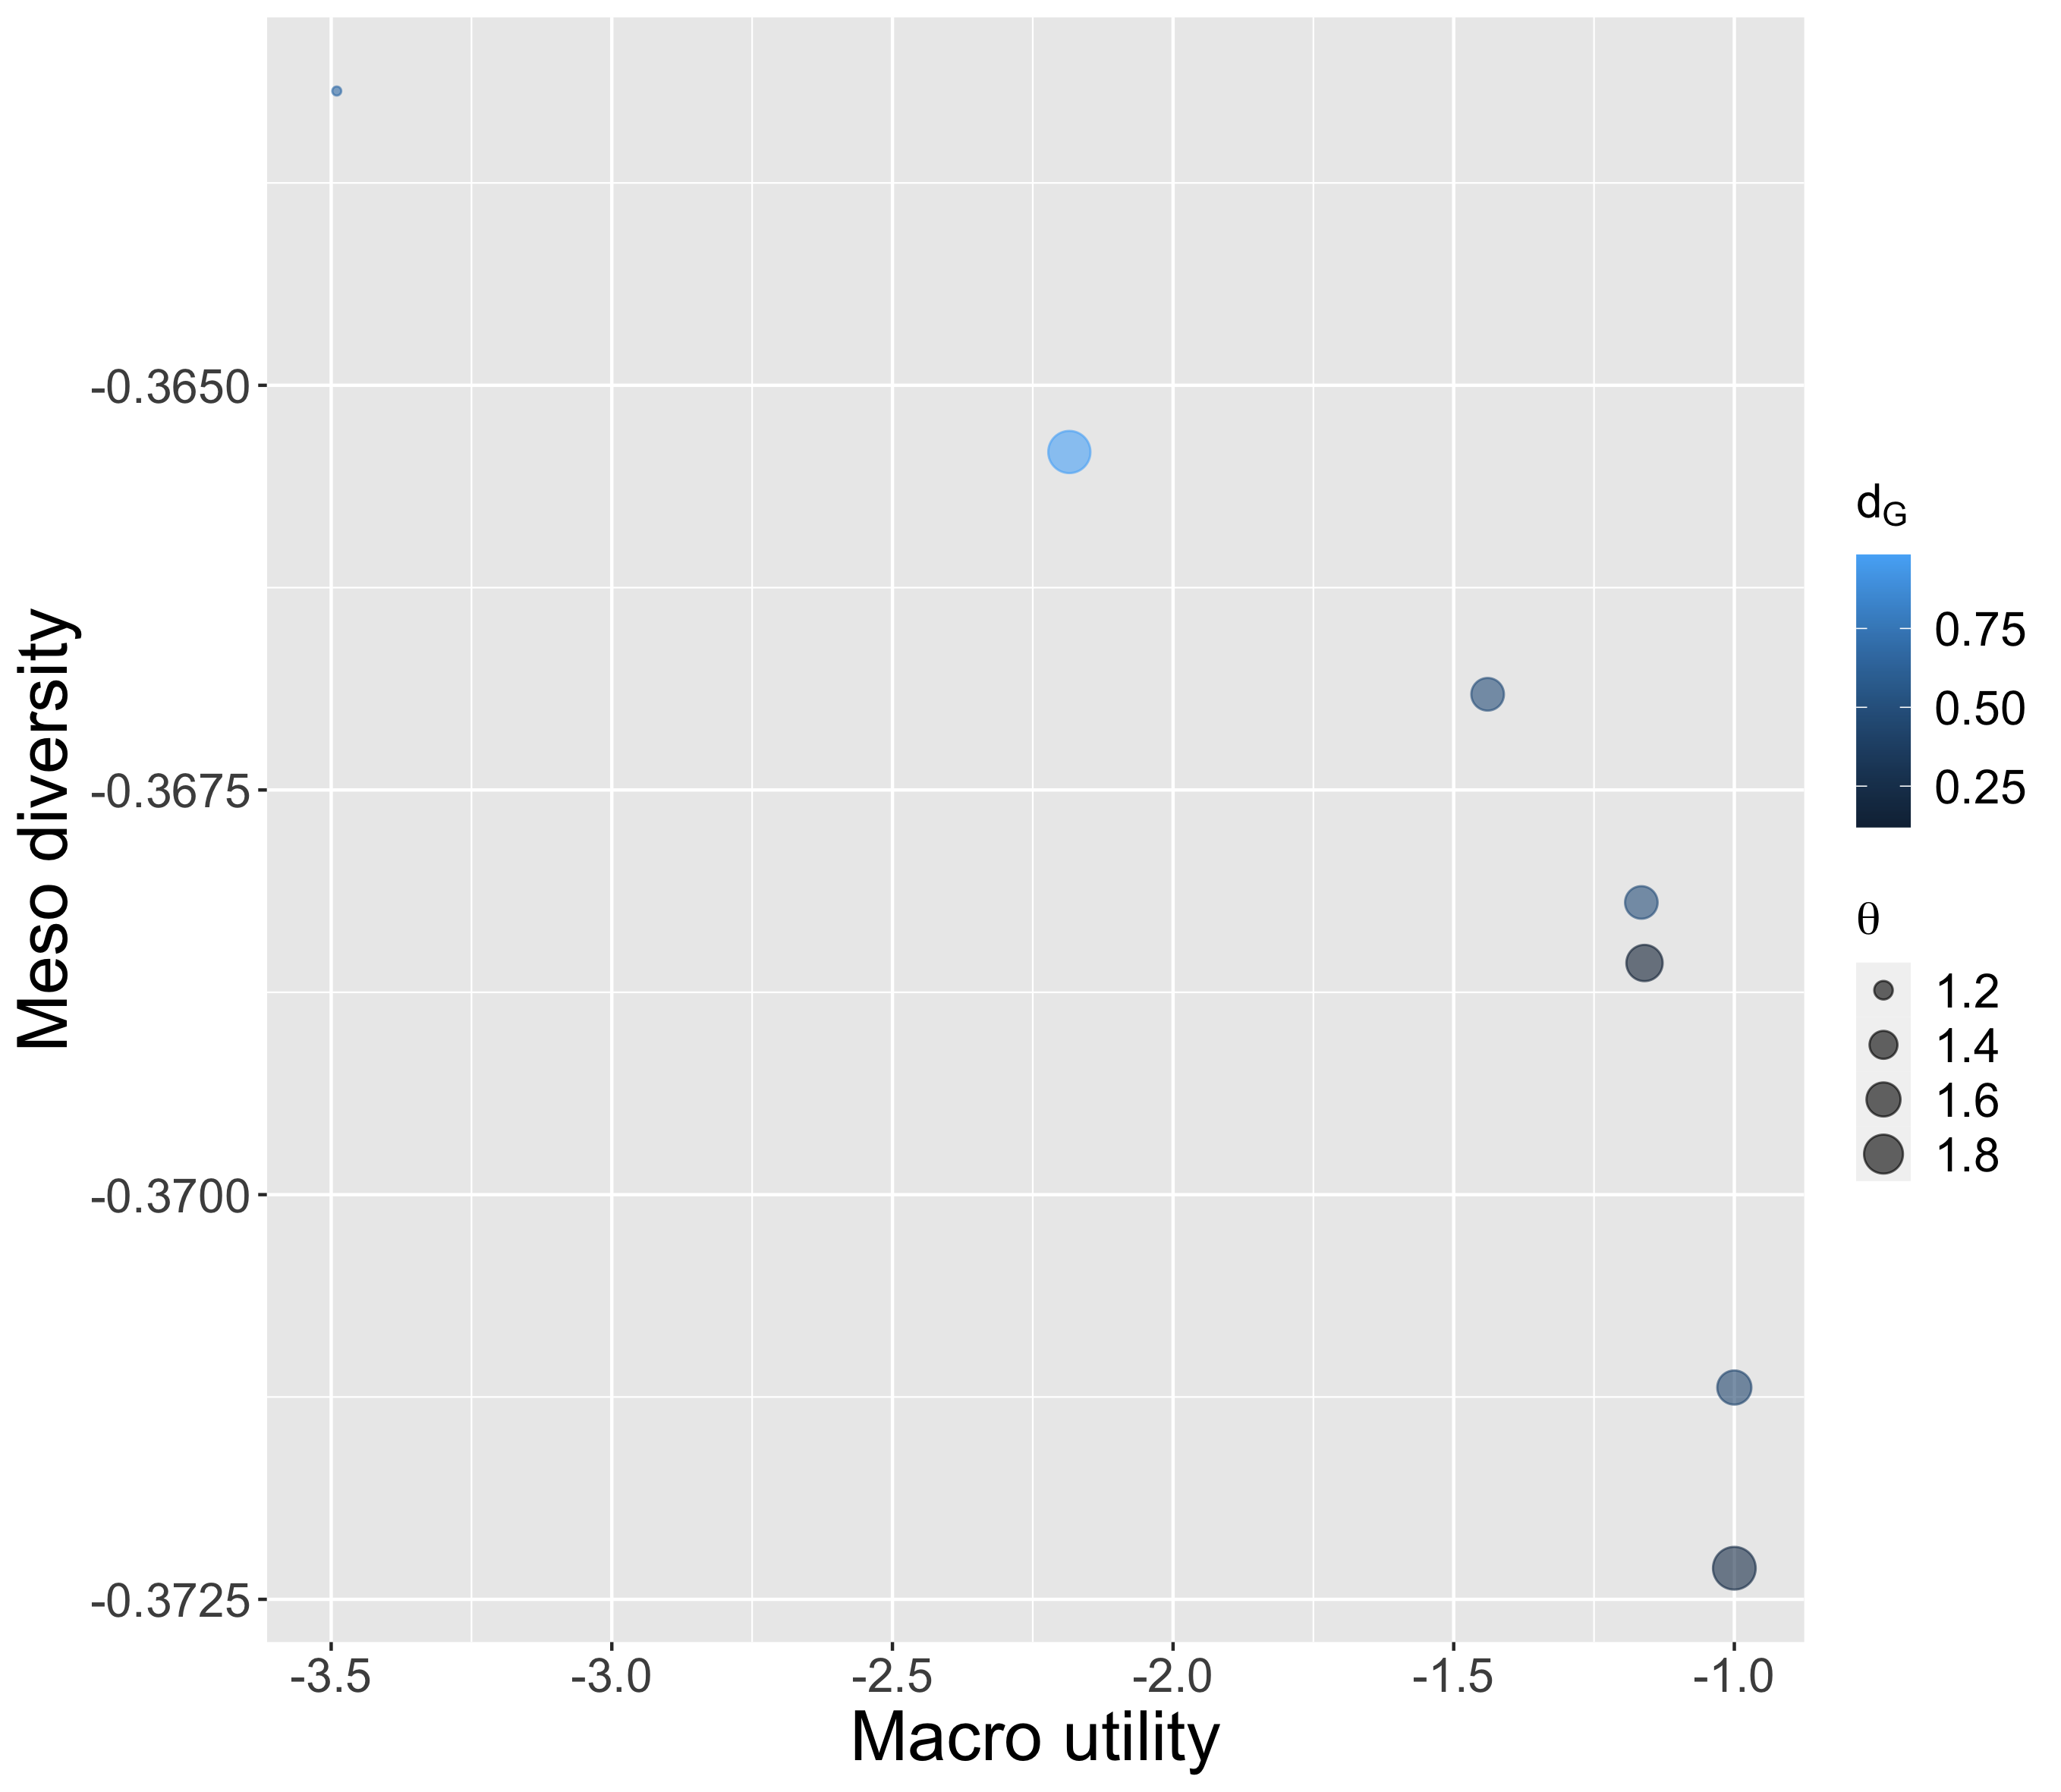
\includegraphics[width=\linewidth]{../figures/paretoDiversity-Fitness_colordG_sizetheta}
    %\caption{Pareto front between the opposite of macro utility and the opposite of meso diversity (both to be minimised to maximise the original objectives). Point color gives interaction distance $d_G$ and point size the innovation threshold $\theta$.\label{fig:pareto}}
 
              
		      }
            \hspace{0.5cm}
            \parbox{0.48\linewidth}{
			    
			    % We find first of all a reduced number of points (10), suggesting that the optimisation is difficult. They however form a Pareto front, with a concave shape - on the contrary to convex fronts generally obtained. This means that extreme points are rather good compromises, witnessing very different regimes which can lead to optima. A middle point corresponds to long interaction distances (large $d_G$), while some points around and on the right extremity of the front are local regimes (small $d_G$), what could be evidence for a detrimental globalisation in that case. It is also a regime where innovation threshold is high, corresponding to a more competitive environment. This optimisation exercise confirms that both scales can be simultaneously taken into account and optimised in policy design.
			    
			    \textbf{Bi-objective optimisation} of indicators at both scales: aggregated utility at the macro scale and diversity of innovations within urban areas; achieved using a \textbf{NSGA2 algorithm} with a population of 200 and for 10,000 generations.

			   
			    \vspace{0.5cm}
			  
			    
			    $\rightarrow$ low number of points on the Pareto front, corresponding to diverse geographical regimes (value of $d_G$ capturing spatial interactions)
			    
			     \vspace{0.5cm}
			    
			     $\rightarrow$ such optimisations can in practice be used to reconcile conflicting stakeholders at different scales
			   
			   \vspace{0.9cm}
			     
		      }
		
		}
		
		
	\end{columns}	
%------------------------------------------------------
%----------------LINE 4--------------------------------
%------------------------------------------------------

	\begin{columns}
		
		\column{0.5}% Width set relative to text width

		
		%==============================================
		\block[titlewidthscale=0.4]{Diversity search}{

            
            \parbox{0.45\linewidth}{
              
              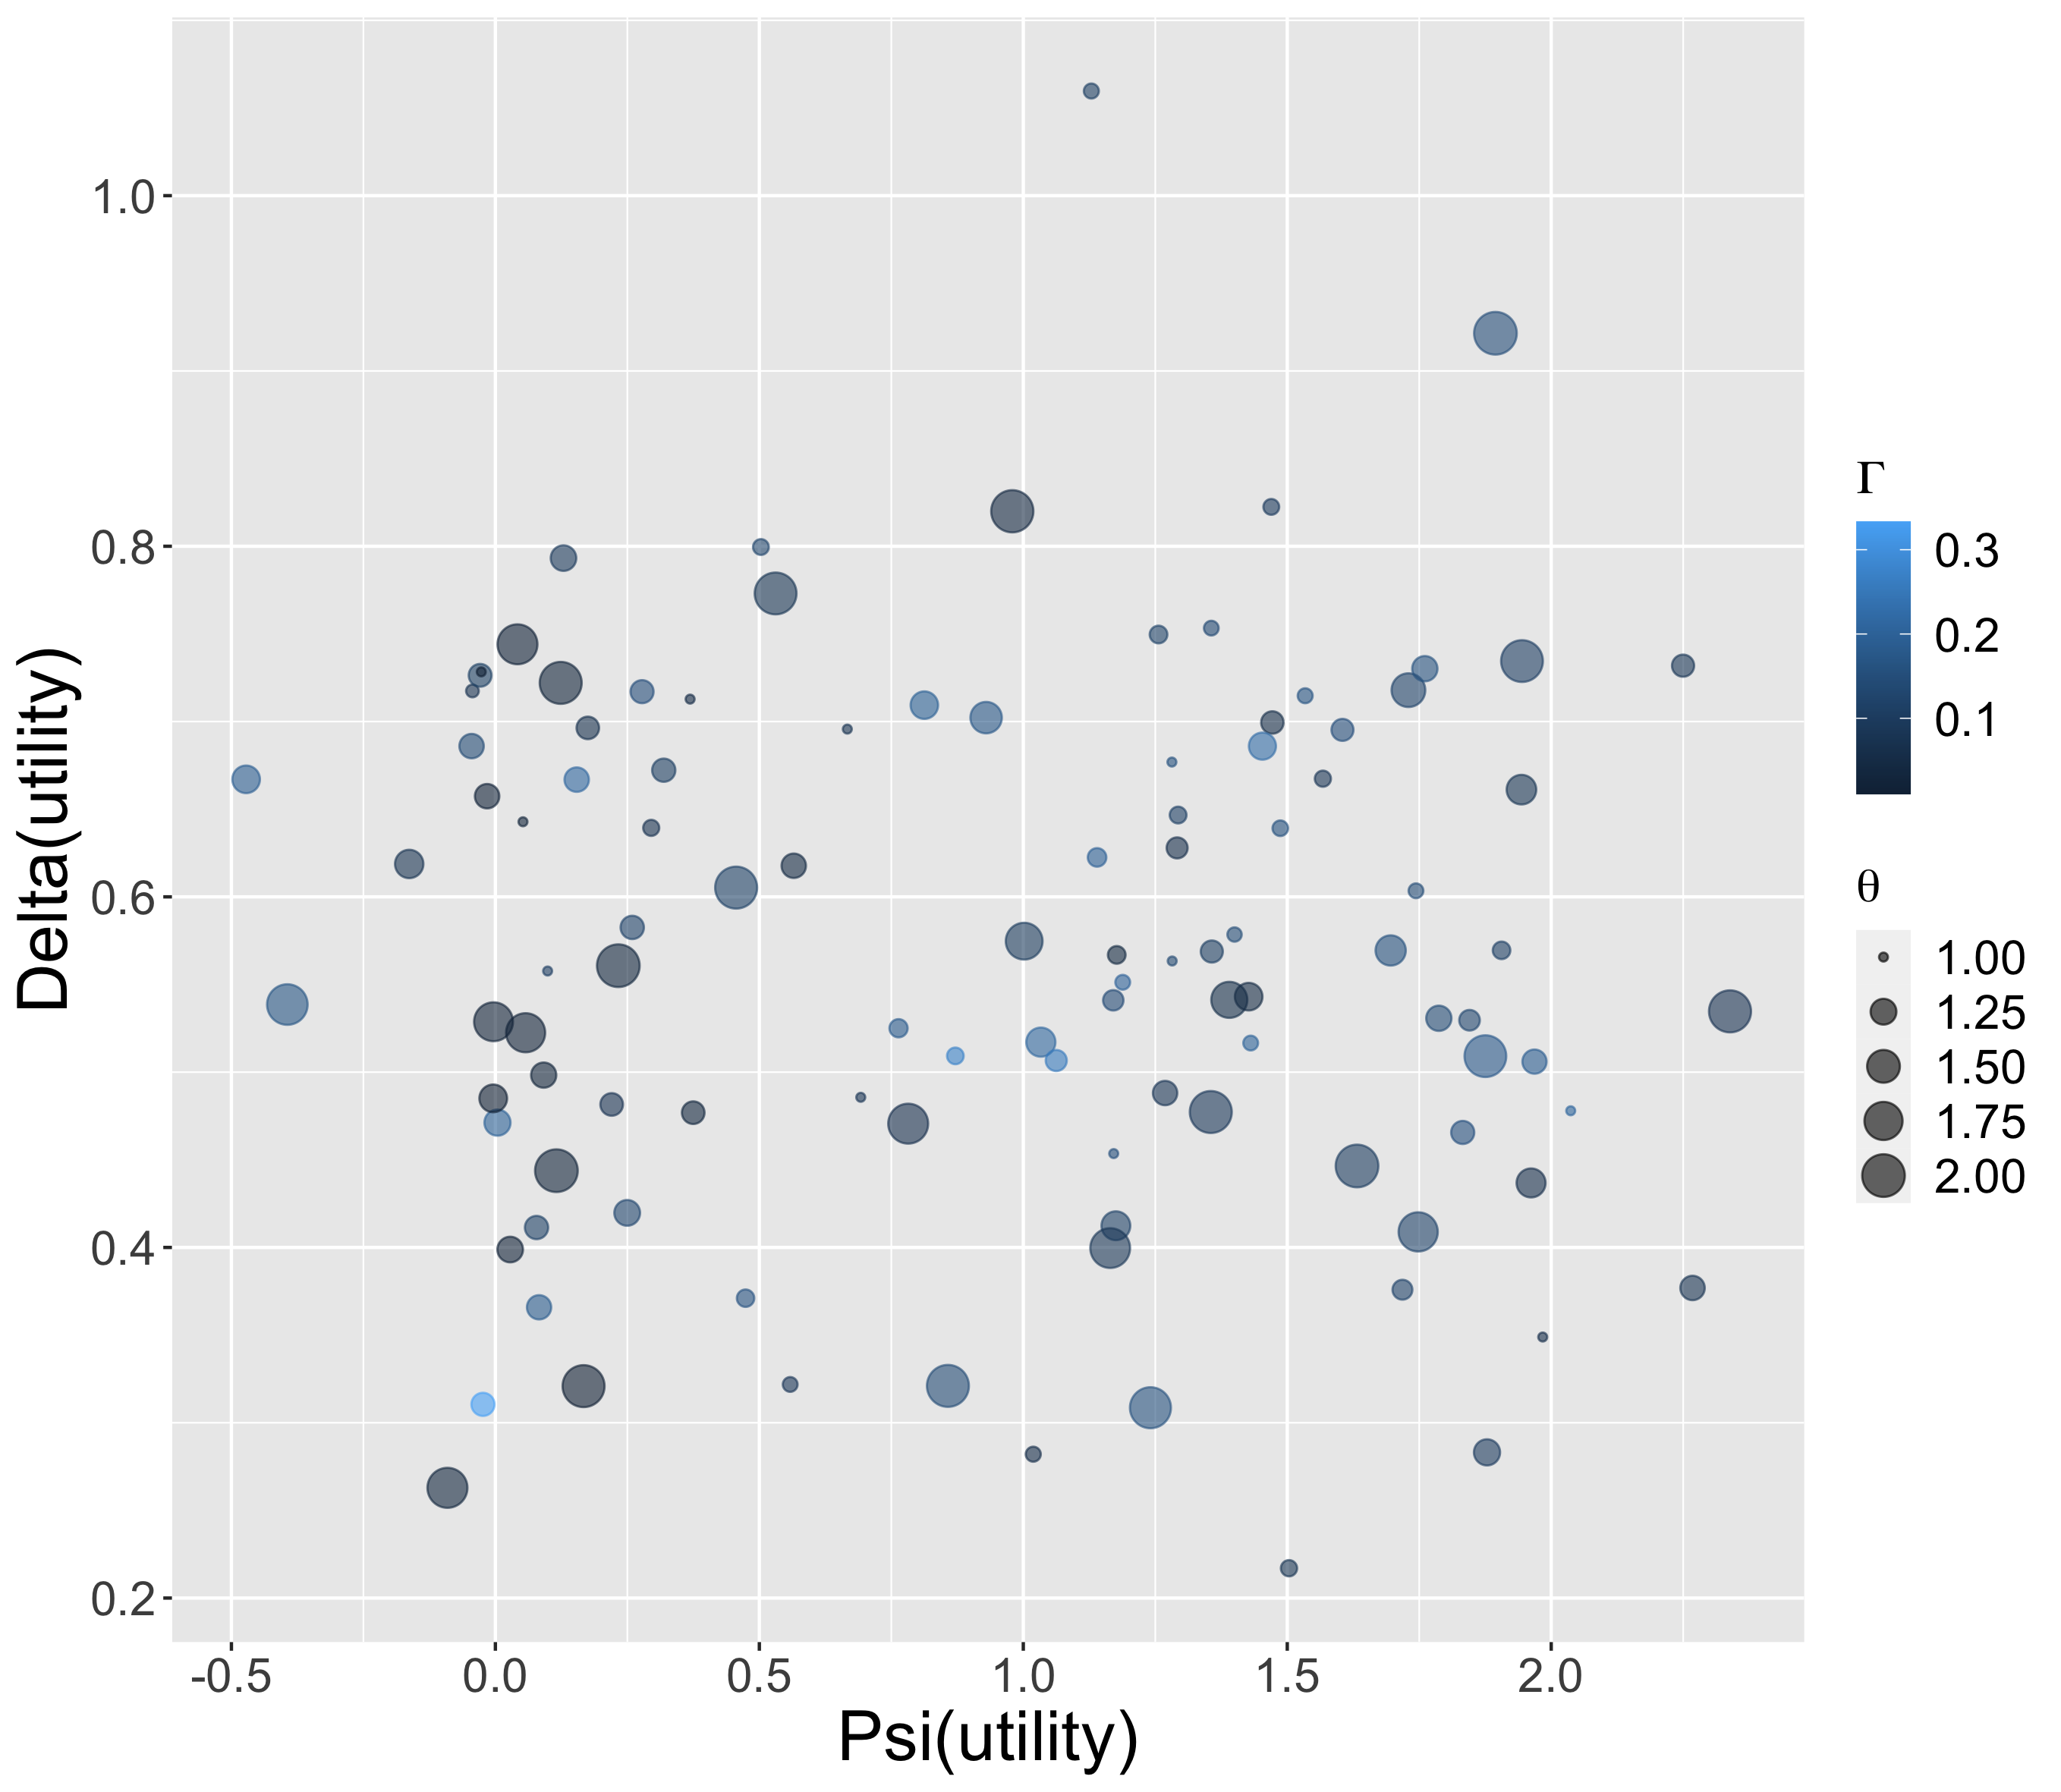
\includegraphics[width=\linewidth]{../figures/pse-psi-delta-utility_colorGamma_sizetheta.png}
    %\textit{Scatter plot between $\Psi (U)$ and $\Delta (U)$, obtained with the PSE diversity search algorithm. Point colour gives $\Gamma (U)$ and point size the innovation threshold $\theta$.}
              
		      }
            \hspace{0.5cm}
            \parbox{0.48\linewidth}{
			    
			    Application of the \textbf{PSE diversity search algorithm} \cite{cherel2015beyond} to obtain the feasible space of emergence regimes.
			    
			    \vspace{0.2cm}
			    
			    % The point cloud obtained is shown in Fig.~\ref{fig:pse}. We find a rather covering cloud, meaning that the model covers a great variety of regimes of emergence. A part of the points are gathered around $\Psi \sim 0$ for varying $\Delta$, corresponding to cases with no causal emergence but downward causation. Several points, disseminated across the cloud, have a value of $\Gamma$ close to 0, implying an autonomy between scale for the positive $\Psi$. $\Delta$ is never negative nor close to 0, meaning that downward causation always occurs, what could have been expected through the explicit top-down feedback process. Altogether, this last experiments confirms that the model captures strong emergence, but also a great variety of causal regimes between scales.
			    
			    $\rightarrow$ downward causation always occurs ($\Delta > 0$)
			    
			     \vspace{0.2cm}
			    
			     $\rightarrow$ many regimes with causal emergence ($\Psi > 0$) and with autonomy between scales ($\Gamma \sim 0$)
			     
			      \vspace{0.2cm}
			     
			     $\rightarrow$ scale coupling is confirmed useful as strong emergence is captured
			     
		      }
            
		}
		%==============================================
		
		% Second column on same line than first one
		\column{0.5}
	    %==============================================
		\block[titlewidthscale=0.4]{Discussion}{

% We have introduced a multi-scalar model for innovation dynamics in systems of cities. Our numerical experiments show, beyond basic model validation and exploration, that (i) contradictory objectives can be optimised through policies across scales, suggesting that this type of approach could further be explored for territorial sustainability; (ii) strong emergence and a great diversity of emergence regimes are captured by the model - confirming the relevance of strongly coupling scale and building such a ``complicated'' model, beyond a single scale.
%Several limits can at this stage be identified, and should be considered for future extensions. The unidimensional innovation space is a strong limitation, keeping the model abstract and difficult to link with data. The economic structure and processes is also very simplified, as we are closer to a phenomenological model. Coupling with economic agent-based models is a perspective for this issue. Regarding the time scales and evolution of urban areas, we also did not include migration of employees - assuming constant team sizes - what is fine with the idea of reinitialised settings at each macro time step, but what would cause more problems if we add memories to companies and employees. In that context, team diversity is crucial for innovation, but the role of sizes and their evolution in time is less clear \citep{hoisl2017r} - so translating population migration directly into firm sizes may not be the best solution. We did not include changes in macro parameters as \cite{raimbault2021strong} does, what could be a way to incorporate more bottom-up feedback in the model.
%Finally, future developments on empirical data would need some model adaptation and complicated data collection and processing work. In particular, finding proxies for innovation, and also collecting firm data which is quite rare, are crucial issues. Such an empirical approach would however be necessary for real-world applications of the model beyond stylised policies.
           
            \vspace{1cm}
            
			\begin{itemize}
				\item Main results: proof-of-concept for a \textbf{bi-objective optimisation across scales}, towards policy applications; \textbf{diversity of emergence regimes} produced by the model
				%\vspace{0.2cm}
				\item Possible extensions and refinements include more detailed economic processes: higher dimension of the innovation space, economic structure for companies, coupling with economic agent-based models, migration of ideas (employees) between urban areas, bottom-up feedback through a change of macro parameters
				%\vspace{0.2cm}
				\item Future application on real urban systems requires innovation data across scales: adaptation of the model to fit specific data, patent data only a proxy of innovation, firm data not open
           
           
           %\vspace{0.5cm}
           
			\end{itemize}
		
		}
		
		
		\end{columns}
		
		%==============================================
		% bibliography managed with natbib
		
		
		
		\block[titlewidthscale=0.4,bodyoffsety=1.8cm,titleoffsety=.1cm]{References}{
			% This command is to prevent the printing of a second "références" in text and to delete white space between block title and bibliography
         
			\renewcommand\refname{\vskip -2cm}
			
            \small
            
   			\begin{multicols}{2}
   			
			\bibliography{../biblio}
			% Plain style so that cited articles appear as number in the poster and are only fully displayed here
			\bibliographystyle{plain}
			
			\end{multicols}
		}
		
		
	
	
	
		
	
	    %==============================================	
	
	
\node [above right,outer sep=20pt,minimum width=\textwidth,align=center,draw=none,fill=none, text = IGNGrisFonce] at (bottomleft) {\centering \huge \bf The 2023 Conference on Artificial Life - 24-28th July, 2023 - Sapporo, Japan};

\end{document}

\endinput


